\documentclass[10pt,a4paper]{amsart}
\usepackage[margin=19mm]{geometry}
\usepackage{amsmath,amssymb,mathtools}
\usepackage[scr=rsfs,cal=euler]{mathalfa}
\usepackage{xfrac}
\usepackage[unicode,hidelinks,bookmarks=false]{hyperref}
\newcommand{\ie}{i.e.\ }
\newcommand{\cf}{cf.\ }
\newcommand{\resp}{respectively\ }
\newcommand{\Subsection}{\subsection}
\providecommand{\nobreakdash}{\nobreak\hbox{-}}
\setlength{\emergencystretch}{2em}
\multlinegap0pt
\usepackage{tikz}
\usepackage{enumerate}
\usepackage{amssymb}
\newtheorem{prop}{Proposition}
\title{Automorphism Groups and Structure of 4-Valent Cayley Graphs on Dihedral Groups}
\author{Amitayu Banerjee}
\date{Source: arXiv:2511.04151v2 (CC BY 4.0)}
\begin{document}
\maketitle

\noindent\emph{Source and licence.} Automorphism Groups and Structure of 4-Valent Cayley Graphs on Dihedral Groups. Version arXiv:2511.04151v2 (CC BY 4.0), distributed by arXiv under the Creative Commons Attribution 4.0 International licence, http://creativecommons.org/licenses/by/4.0/, as recorded in the arXiv licence metadata for this exact version and shown on the abstract page https://arxiv.org/abs/2511.04151v2. Full licence notice: \texttt{licenses/arxiv-2511.04151-CC-BY-4.0.txt}.\par\smallskip

\noindent\textit{Editorial scope.} Counted unit: the article's prop 3.1 (source0.tex lines 283--302). The article's complete original proof of it is delivered with it (source0.tex lines 304--406, one \texttt{proof} environment of 103 lines). No mathematics is written, repaired or re-derived: the statement and the proof are the article's own lines, in the article's own notation, and no retained line is substituted or re-flowed.  No further source-local context is needed: every cross-reference of every retained line resolves inside the two delivered spans.  Nothing was omitted from any retained span, so the package carries no omission record.  No retained line contains a citation, so the wrapper carries no bibliography and no bibliography entry.  The retained lines contain the article's own diagram code, which the wrapper typesets with the standard tikz packages; no image file is delivered and the package declares no asset dependency.  Editorial formatting only, in addition: an AMS \texttt{amsart} preamble that restates the article's own declarations and macros used by the retained lines, namely the environments \texttt{prop} on separate counters, together with the standard packages those lines need.  The retained environments print in this document as Proposition 1 in order of appearance, whereas the article prints the same items with the numbering of its own full document.  The complete native source of the article as distributed in the arXiv e-print for this exact version is bundled unchanged as \texttt{sources/188565/source0.tex}.
\begin{prop}\label{Proposition 3.1}
{\em
Assume $S\subseteq R_{n}\setminus\{e\}$ is an inverse-closed subset of rotations of $D_{2n}$ with $|S|=2k<n$ for some $k\ge2$.  
Choose representatives $a_1,\dots,a_k\in\mathbb{Z}_n$ such that 
$S=\{r^{\pm a_1},\dots,r^{\pm a_k}\}$.
Let $T = \{\pm a_1, \dots, \pm a_k\}$, 
$G_{1} = \mathrm{Cay}(D_{2n}, S)$, 
$G_{2} = \mathrm{Cay}(\mathbb{Z}_n, T)$, and $d = \gcd(n, a_1, \dots, a_k)$. Then:
\begin{enumerate}
  \item $\mathrm{Cay}(D_{2n}, S) \;\cong\; \mathrm{Cay}(\mathbb{Z}_n, T) + \mathrm{Cay}(\mathbb{Z}_n, T)$.
  
  \item If $d = 1$, then $G_{2}$ is connected. So $G_{1}$ has $2$ components isomorphic to $G_{2}$.
  
  \item If $d > 1$, write $n = d n'$ and $a_i = d a_i'$ for all $i$, and set 
  $T' = \{\pm a_1', \dots, \pm a_k'\} \subset \mathbb{Z}_{n'}$. 
  Then $G_{2}$ decomposes into $d$ components isomorphic to $\mathrm{Cay}(\mathbb{Z}_{n'}, T')$. 
  So, $G_{1} \cong G_{2} + G_{2}$ splits into $2d$ components isomorphic to $\mathrm{Cay}(\mathbb{Z}_{n'}, T')$.
\end{enumerate}
}
\end{prop}

\begin{proof}
(1). The vertex set of $\mathrm{Cay}(D_{2n}, S)$ is $D_{2n} = R_{n} \cup F_{n}$.  
For any rotation $r^t \in R_{n}$, 
if $g \in R_{n}$, then $g r^t \in R_{n}$, while if $g \in F_{n}$, then $g r^t \in F_{n}$.  
Thus, every edge $\{ g, g r^t \}$ produced by a rotation generator $r^{t}\in S$ is an intra-layer edge.  
Consequently, no generator in $S$ produces an edge joining $R_{n}$ to $F_{n}$.  
Therefore, $\mathrm{Cay}(D_{2n}, S)$ splits into two vertex-disjoint subgraphs induced on $R_{n}$ and on $F_{n}$.
Consider the induced subgraph $\Gamma_{R_{n}}$ of $\mathrm{Cay}(D_{2n}, S)$ on $R_{n}$.  
If $t \in T$, then $\Gamma_{R_{n}}$ contains the edge $\{ r^i, r^{i+t} \}$.  
Hence $\Gamma_{R_{n}}\cong\mathrm{Cay}(\mathbb{Z}_n, T)$.  
Similarly, the induced subgraph $\Gamma_{F_{n}}$ on $F_{n}$ is isomorphic to $\mathrm{Cay}(\mathbb{Z}_n, T)$.  
In particular, the map $\varphi : R_{n} \to F_{n}$ defined by $\varphi(r^i) = s r^i$ is a bijection, and for any $t \in T$,
$\{ \varphi(r^i), \varphi(r^{i+t}) \}
= \{ s r^i, s r^{i+t} \}
= \{ s r^i, (s r^i) r^t \}$.
Thus, edges inside $R_{n}$ correspond exactly to edges inside $F_{n}$ under $\varphi$, so $\Gamma_{F_{n}} \cong \Gamma_{R_{n}}$.  
Consequently,
$\mathrm{Cay}(D_{2n}, S)
= \Gamma_{R_{n}} + \Gamma_{F_{n}} 
\;\cong\;
\mathrm{Cay}(\mathbb{Z}_n, T) + \mathrm{Cay}(\mathbb{Z}_n, T)$.


%%%%%%%%%%%%%%%%%%%%%%%%%%%%%%%%%%%%%%%%%%%%%
\begin{figure}[h]
\centering
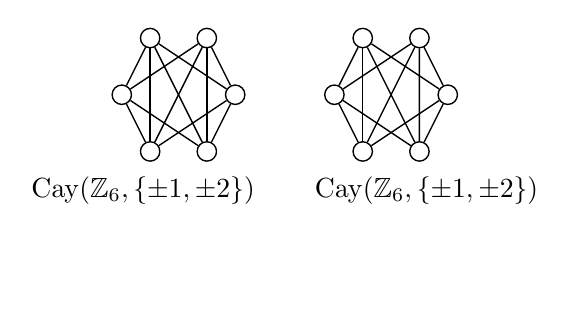
\begin{tikzpicture}[
    scale=0.45,
    every node/.style={circle,draw,fill=white,inner sep=1pt,minimum size=7pt},
    line width=0.5pt
]

% Function to draw K_{2,2,2} with unique index (#1) and x-shift (#2)
\newcommand{\Ktwotwotwo}[2]{
  \def\i{#1}
  \def\xshift{#2}
  \def\dx{1.0}

  % A-part (top)
  \node (A1\i) at (\xshift-0.8*\dx, 1.6) {};
  \node (A2\i) at (\xshift+0.8*\dx, 1.6) {};

  % B-part (middle)
  \node (B1\i) at (\xshift-1.6*\dx, 0) {};
  \node (B2\i) at (\xshift+1.6*\dx, 0) {};

  % C-part (bottom)
  \node (C1\i) at (\xshift-0.8*\dx,-1.6) {};
  \node (C2\i) at (\xshift+0.8*\dx,-1.6) {};

  % Edges between parts
  \foreach \u in {A1\i,A2\i}{
    \foreach \v in {B1\i,B2\i,C1\i,C2\i}{
      \draw (\u)--(\v);
    }
  }
  \foreach \u in {B1\i,B2\i}{
    \foreach \v in {C1\i,C2\i}{
      \draw (\u)--(\v);
    }
  }
}

% ---------- Draw both ----------
\Ktwotwotwo{1}{0}    % left copy
\Ktwotwotwo{2}{6.0}  % right copy

% Labels
\node[draw=none,fill=none] at (-1,-2.7)
  {$\mathrm{Cay}(\mathbb{Z}_{6},\{\pm1,\pm2\})$};
\node[draw=none,fill=none] at (7,-2.7)
  {$\mathrm{Cay}(\mathbb{Z}_{6},\{\pm1,\pm2\})$};

\end{tikzpicture}
\vspace{-4.5em}
\caption{\em The graph $\mathrm{Cay}(D_{12}, \{r^{\pm1}, r^{\pm2}\})$ is the disjoint union $K_{2,2,2} + K_{2,2,2}$.}
\end{figure}

%%%%%%%%%%%%%%%%%%%%%%%%%%%%%%%%%%%%%%%%%%%%%

(2). We know that $\mathrm{Cay}(\mathbb{Z}_n, T)$ is connected if and only if $T$ is a generating set of $\mathbb{Z}_{n}$.  
The subgroup generated by $T$ is 
$\langle T \rangle$ = $\{ x_1 a_1 + \cdots + x_k a_k \pmod{n} : x_i \in \mathbb{Z} \}$
= $d \mathbb{Z}_n$
= $\{ 0, d, 2d, \dots, n - d \}$.  
Hence $\mathrm{Cay}(\mathbb{Z}_n, T)$ is connected if and only if $\langle T \rangle = \mathbb{Z}_n$, which is equivalent to $d=\gcd(n, a_1, \dots, a_k) = 1$.

(3). We recall that $d = \gcd(n, a_1, \dots, a_k)$, $n = d n'$, $a_i = d a_i'$ for $i = 1, \dots, k$.  
Let $\{ C_j : 0 \le j \le d-1 \}$ be a partition of $\mathbb{Z}_{n}$ where 
$C_j = \{j + k d : k = 0, \dots, n'-1\}$.
The graph $G_2$ is the disjoint union of induced subgraphs on $C_j$'s.  
In particular, if $x \in C_j$ and $t \in T$, then $t$ is a multiple of $d$ (since each $a_i$ is).  
Thus, $x + t \in C_j$ since $x + t \equiv x \pmod{d}$.  
Consequently, no edge $\{ x, x + t \}$ joins $C_i$ and $C_j$ for $i \ne j$.
Fix $0 \le j \le d-1$.  
The map 
$\psi_j : C_j \to \mathbb{Z}_{n'}, \psi_j(j + k d) \equiv k \pmod{n'}$,
is a graph isomorphism from the induced subgraph on $C_j$ to 
$\mathrm{Cay}(\mathbb{Z}_{n'}, T')$,  
where $T' = \{\pm a_1', \dots, \pm a_k'\}$.  
Therefore, there are exactly $d$ identical components, each isomorphic to $\mathrm{Cay}(\mathbb{Z}_{n'}, T')$.  
Since $\gcd(n', a_1', \dots, a_k') = 1$, $\langle T' \rangle = \mathbb{Z}_{n'}$, and thus $\mathrm{Cay}(\mathbb{Z}_{n'}, T')$ is connected.  
\end{proof}

\end{document}
